\section{Pohyb hmotného bodu v priestore}
\label{sec:HB}
Majme hmotný bod, ktorý sa pohybuje v priestore a je opísaný nasledovnými diskrétnymi rovnicami:
\label{math:model_HB}
\begin{subequations}
	\begin{align}
	&x_{k+1}^{(1)} = x_{k}^{(1)} + x_{k}^{(2)} + u_{k},\\
	&x_{k+1}^{(2)} = x_{k}^{(2)} + 0,5u_{k}.
	\end{align}
	\end{subequations}
Prvý stav $x^{(1)}$ predstavuje polohu v $[m]$, druhý stav $x^{(2)}$ predstavuje rýchlosť v $[m s^{-1}]$ a vstup do systému $u$ predstavuje zrýchlenie hmotného bodu. Pomocou týchto rovníc si môžeme zostrojiť maticu stavov $A$ a maticu vstupov $B$:
\begin{align}
A = \begin{bmatrix}
1 &1\\
0 &1
\end{bmatrix},
B= \begin{bmatrix}
1\\
0,5
\end{bmatrix},
\end{align}
a následne ich dosadíme do lineárneho stavového opisu systému:
\begin{align}
& x_{k+1} = Ax_{k}+Bu_{k}.
\end{align}
Takto zostrojený model systému využijeme pri návrhu lineárneho MPC s predikčným horizontom $N = 5$, podľa teórie uvedenej v kapitole \hyperref[subse:MPC]{(2.1.1)}. S nasledovnými váhovými maticami:
\begin{align}
Q = \begin{bmatrix}
1&0\\
0&1
\end{bmatrix}, 
R = \begin{bmatrix}
1
\end{bmatrix}.
\end{align}
Následne si rozdistribuujeme a upravíme takto navrhnuté MPC na $N = 5$ predikčných horizontov podľa postupu, ktorý sme si uviedli v kapitole \hyperref[subse:Lin_MPC_ADMM]{(2.4.1)}. Ako kritériá pre zastavenie \hyperref[subse:ADMM2]{iterácií v ADMM} sme zvolili presnosť hľadaných počiatočných stavov $\norm{\tilde{H}_{1}U_{k-1} + \tilde{H}_{2}U_{k} - \tilde{A}U_{k-1}} < \epsilon,\hspace{0.5cm} k=1,\dots,N-1$ (veľkosť duálnej funkcie) a taktiež veľkosť zmeny predikovaných akčných zásahov $\norm{U(1)_{k}^{(i-1)}-U(1)_{k}^{(i)}} < \epsilon,\hspace{0.5cm} k=0,\dots,N-1$, kde $\epsilon = 1\mathrm{e}{-5}$. Akonáhle sa jedna z týchto podmienok splní, môžeme prehlásiť, že sme našli optimálne akčné zásahy. Rovnako, ako v obyčajnom MPC, zoberieme prvý akčný zásah $u_{0}$, aplikujeme ho a ostatné zahodíme. Tento postup opakujeme, pokiaľ neskonvergujeme do optima (odchýlka stavov rovná nule, alebo sa dostaneme na žiadanú hodnotu).

Vytvorili sme simuláciu na modeli uvedenom v rovniciach \hyperref[math:model_HB]{(3.1)}, aby sme boli schopní porovnať normálne MPC s decentralizovaným MPC. Záporné hodnoty budú hovoriť o pohybe v opačnom smere. 
\begin{figure}[H]
	\centering
	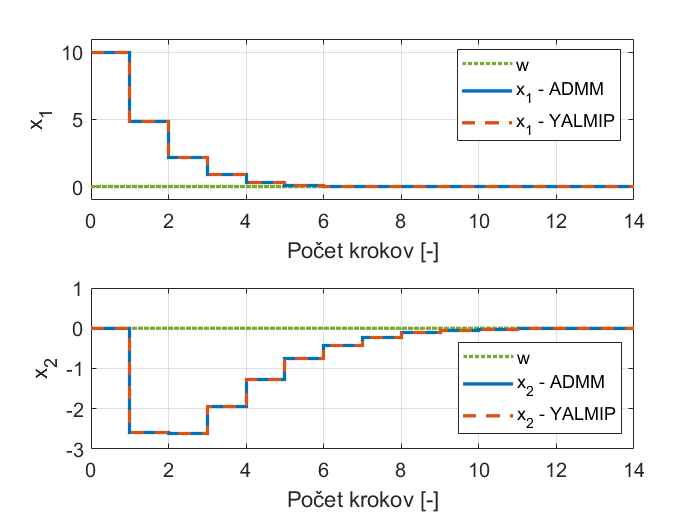
\includegraphics[width=13cm,height=10cm]{images/Hmotny_bod/Priebeh_riadenia}
	\caption{Priebeh riadenia pre lineárny systém}
	\label{fig1: PRLS}
\end{figure}
Ako môžeme vidieť na (Obr. 3.1), v oboch prípadoch sa nám podarilo dosiahnuť žiadanú veličinu (nulovú odchýlku stavov) a priebeh riadenia ja totožný pri oboch metódach.
\newpage
\begin{figure}[H]
	\centering
	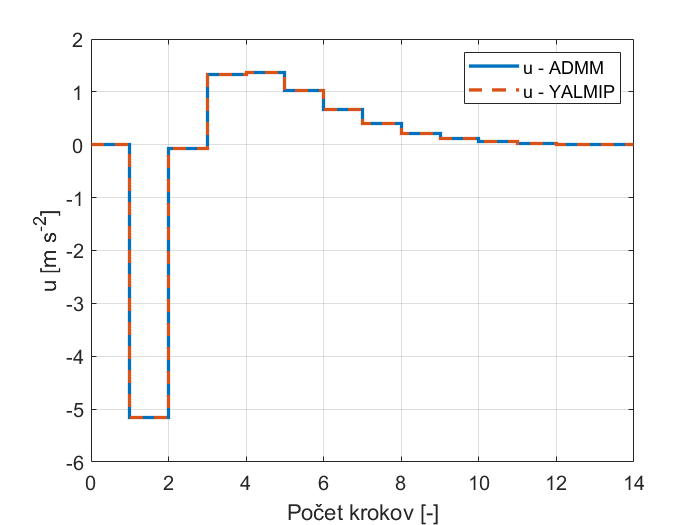
\includegraphics[width=13cm,height=10cm]{images/Hmotny_bod/Akcne_zasahy}
	\caption{Vývoj akčných zásahov}
	\label{fig2:AZLS}
\end{figure}
Rovnako ako stavy, tak aj akčné zásahy, sú totožné pri oboch metódach, čo môžeme vidieť na (Obr. 3.2).
\newpage
\begin{figure}[H]
	\centering
	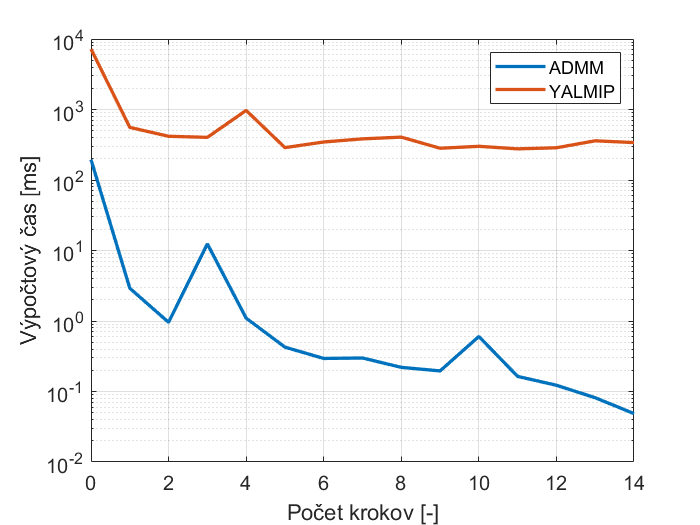
\includegraphics[width=13cm,height=10cm]{images/Hmotny_bod/Vypoctovy_cas}
	\caption{Porovnanie výpočtovej náročnosti MPC, medzi ADMM a YALMIP}
	\label{fig3: VNAA}
\end{figure}
Pre nás je najdôležitejší graf výpočtovej náročnosti (Obr. 3.3). Ako môžeme vidieť, podarilo sa nám dosiahnuť značné zlepšenie oproti analytickému riešiteľu z toolboxu YALMIP. Zatiaľ čo inicializačný čas pre ADMM bol okolo 100ms, najrýchlejšie riešenie pomocou YALMIP sa pohybovalo vyššie ako 100ms. Z tohoto porovnania vyplýva, že ADMM metóda je lepšia pre systémy s rýchlou dynamikou, ak sú opísané lineárnym matematickým modelom. 
\newpage